\documentclass{standalone}

%--------------------------------------------------------------------------------------------------------
% PAQUETES
%--------------------------------------------------------------------------------------------------------

\usepackage{tikz}
\usepackage{tkz-euclide}
\usepackage{siunitx}
\usepackage{fourier}

%--------------------------------------------------------------------------------------------------------
% OTRAS CONFIGURACIONES
%--------------------------------------------------------------------------------------------------------

\usetkzobj{all}

%--------------------------------------------------------------------------------------------------------
% INICIO DEL DOCUMENTO
%--------------------------------------------------------------------------------------------------------

\begin{document}
	
	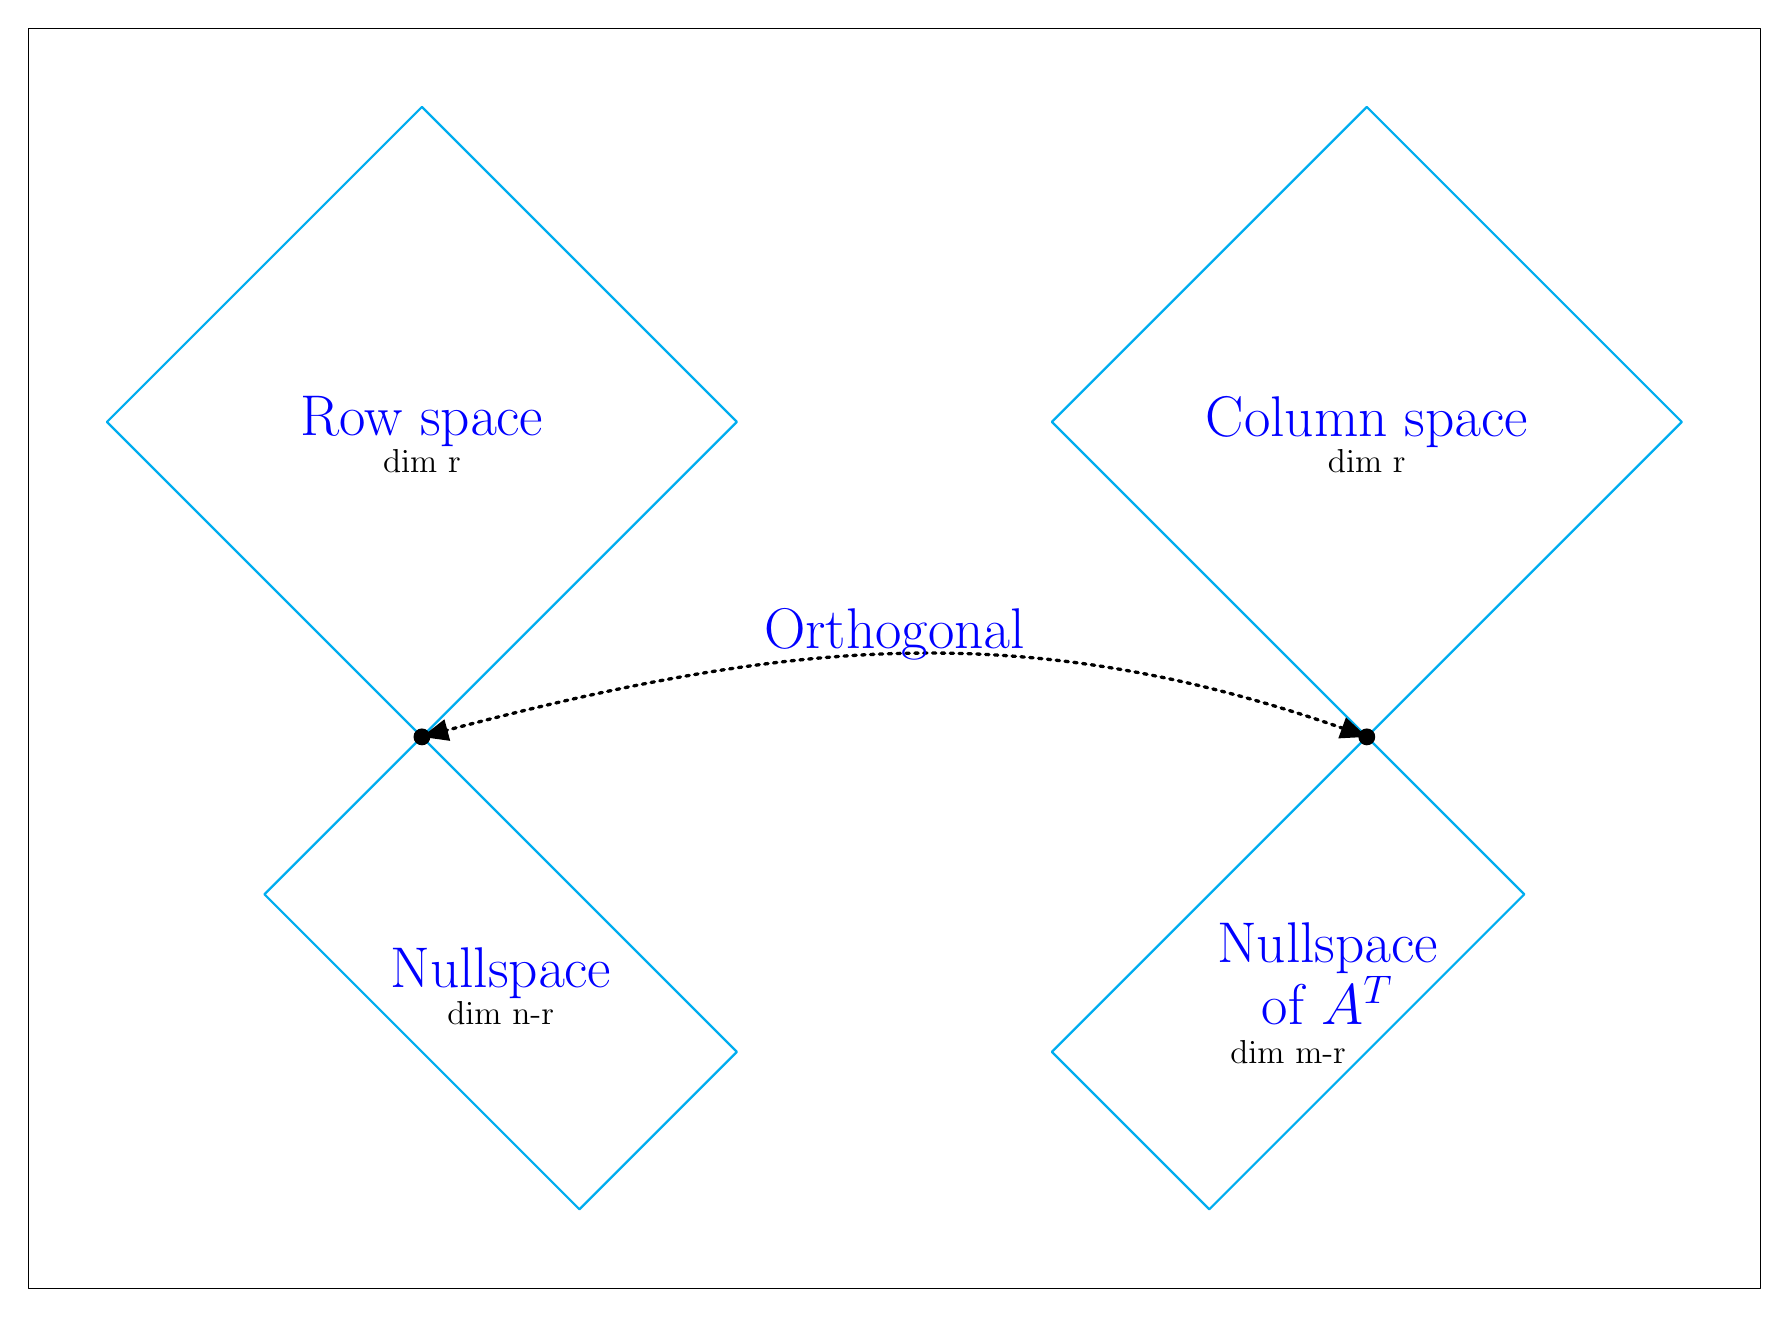
\begin{tikzpicture}[line cap = round, line join = round, >=triangle 45]
		%\draw[red] (-1,-1) grid (20,18);
		%\draw[blue] (0,0) circle (1mm);
		
		% Nullspace of A
		\draw [cyan, thick](6,1) --(8,3)--(4,7)--(2,5)  -- cycle;
		\node [blue] at (5,4) {\huge Nullspace}; Dim(N(A))=n-r
		\node   at (5,3.5) {\large dim n-r}; 
		% Rowspace of A
		\draw [cyan, thick](4,7)--(8,11)--(4,15)--(0,11)  -- cycle;
		\node [blue] at (4,11) {\huge Row space};
		\node  at (4,10.5) {\large dim r}; 
		% Intersection between Nullspace and Rowspace
		\draw [fill=black] (4,7) circle (1mm);

		% Nullspace of A^T
		\draw [cyan, thick](12,3) --(14,1)--(18,5)--(16,7)  -- cycle;
		\node [align=center,blue] at (15.5,4) {\huge Nullspace \\ \huge of $A^T$};
		\node  at (15,3) {\large dim m-r}; 
		% Column space of A
		\draw [cyan, thick](16,7)--(20,11)--(16,15)--(12,11)  -- cycle;
		\node [blue] at (16,11) {\huge Column space};
		\node  at (16,10.5) {\large dim r}; 
		% Intersection between Nullspace of A^T and Rowspace
		\draw [fill=black] (16,7) circle (1mm);
		
		
		% orthogonal 
		%\draw [<->,dotted] (4,7) -- (5.333,7.3950)-- (6.667,7.6913)-- (8,7.8889)-- (9.3333,7.8977)-- (12,7.8889)-- (13.3333,7.6913)-- (14.6667,7.3950)-- (16,7);
		\draw[<->,dotted,very thick] (4,7) to [out=15, in=160] (16,7);
		\node [blue] at (10,8.3) {\huge Orthogonal};
		\draw  (-1,0) rectangle (21,16); % to frame the images
	\end{tikzpicture}

\end{document}